\documentclass[10pt,a4paper,twocolumn]{article}
\usepackage[margin=1.45cm,top=1.35cm,bottom=1.4cm]{geometry}
\usepackage{amsmath,amssymb,graphicx,booktabs,xcolor,microtype,hyperref}
\usepackage{titlesec,caption}
\definecolor{teal}{HTML}{087F8C}
\definecolor{ink}{HTML}{182B40}
\hypersetup{colorlinks=true,urlcolor=teal,citecolor=teal,linkcolor=teal,pdftitle={PrivacyGuard: RL for adaptive data sharing},pdfauthor={Patel Jaimil Nareshkumar and Nitin Koronde R.}}
\setlength{\columnsep}{0.55cm}
\setlength{\parindent}{0pt}
\setlength{\parskip}{3pt}
\setlength{\textfloatsep}{6pt}
\setlength{\floatsep}{5pt}
\renewcommand{\dbltopfraction}{.75}
\renewcommand{\textfraction}{.1}
\captionsetup{font=small,labelfont=bf,skip=3pt}
\titleformat{\section}{\normalsize\bfseries\color{teal}}{\thesection}{.5em}{}
\titlespacing*{\section}{0pt}{6pt}{3pt}
% Supplied by the user. Replace the account-profile note with a VERIFIED repository URL after publishing.
\newcommand{\TeamNames}{Patel Jaimil Nareshkumar (B23CH1029)\quad\textbullet\quad Nitin Koronde R. (B23CH1028)}
\newcommand{\RepositoryLine}{GitHub account: \href{https://github.com/JaimilNPatel}{github.com/JaimilNPatel}\quad\textit{Project repository publication pending}}

% Generated by python -m privacyguard.report_assets; do not type experimental numbers here.
\newcommand{\QReturn}{18.23}
\newcommand{\QCI}{0.12}
\newcommand{\GreedyReturn}{13.48}
\newcommand{\GainPercent}{35.26}
\newcommand{\OptPercent}{95.98}
\newcommand{\OptValue}{19.00}
\newcommand{\GapValue}{0.76}
\newcommand{\PairedGain}{4.75}
\newcommand{\PairedCI}{0.08}
\newcommand{\FatigueGain}{0.05}
\newcommand{\FatigueCI}{0.06}
\newcommand{\ResultsRows}{%
Q-learning & $18.23\pm0.12$ & 23.76 & 9.48 \\
SARSA & $17.91\pm0.14$ & 23.45 & 9.61 \\
Myopic Q & $12.90\pm0.12$ & 19.27 & 9.98 \\
No budget obs. & $12.09\pm0.39$ & 19.26 & 9.96 \\
No fatigue obs. & $18.18\pm0.09$ & 23.71 & 9.50 \\
Greedy & $13.48\pm0.11$ & 20.17 & 9.98 \\
Always coarse & $8.73\pm0.06$ & 14.77 & 10.00 \\
Exact DP & $19.02\pm0.10$ & 24.52 & 9.29 \\
}

\newcommand{\ind}{\mathbf{1}}
\pagestyle{plain}
\begin{document}
\twocolumn[{
{\color{teal}\small\bfseries AI COURSE MINI-PROJECT\hfill REINFORCEMENT LEARNING}
\vspace{3pt}
\begin{center}
{\LARGE\bfseries\color{ink} PrivacyGuard}\\[3pt]
{\large RL for adaptive data-sharing decisions}\\[6pt]
{\small\TeamNames}\\[3pt]
{\footnotesize\RepositoryLine}
\end{center}
\vspace{1pt}\hrule\vspace{7pt}
}]
\small
\textbf{Abstract.} PrivacyGuard learns when to share full data, provide a coarse response, ask for consent, or deny access. A finite exposure budget and consent fatigue give decisions delayed consequences. We implement tabular Q-learning with a hard permission/budget guard and evaluate eight independent runs against SARSA, planning/observation ablations, reference strategies, and an analytical ceiling. On held-out synthetic sessions, Q-learning improves return by \GainPercent\% over greedy sharing and attains \OptPercent\% of the model optimum. A saved-policy demo exposes Q values, training counts, and session audits.

\section{Problem and sequential motivation}
An assistant handling location, spending, or activity requests must balance task value with disclosure. A low-value disclosure now may consume budget needed later; repeated consent prompts can reduce later acceptance. This is sequential control without labelled correct actions. Context-sensitive handling is motivated by contextual integrity~\cite{nissenbaum}; our numerical costs are explicit synthetic assumptions.

\textbf{Project contribution.} We integrate exposure allocation, stochastic consent, action-induced fatigue, and permission enforcement in a small explainable MDP. Multiseed ablations, an exact diagnostic, and an offline demo provide an auditable evaluation. We do not claim a new RL algorithm or established research novelty.

\section{RL formulation and cost model}
\textbf{State space.} The six-component observation is $s=(h,b,f,u,d,p)$: requests remaining $h\in\{0,\ldots,12\}$, exposure budget $b\in\{0,\ldots,10\}$, consent fatigue $f\in\{0,1,2\}$, utility and sensitivity indices $u,d\in\{0,1,2\}$, and standing full-permission bit $p\in\{0,1\}$. There are $13\cdot11\cdot3\cdot3\cdot3\cdot2=7{,}722$ combinations including terminal states, $7{,}128$ nonterminal combinations, and $30{,}888$ Q entries. Sessions start at $(h,b,f)=(12,10,0)$ and end at $h=0$.

\textbf{Request dynamics.} Utility is $U=(1,3,7)_u$ and full exposure is $E=(1,2,4)_d$. New contexts are independent draws with marginals $P(u)=P(d)=(.45,.35,.20)$ and $P(p)=(.40,.60)$. With realised exposure $e$, $b'=b-e$ and $h'=h-1$. Asking gives $f'=\min(2,f+1)$; any other action gives $f'=\max(0,f-1)$. This observation contains the history needed by the assumed dynamics, satisfying the Markov property.

\textbf{Actions and hard guard.} $\mathcal A=\{\text{deny},\text{coarse},\text{ask},\text{full}\}$. Full requires $p=1$ and $b\ge E$; coarse requires $b\ge\lceil.35E\rceil$; ask requires $b\ge E$ so acceptance can be honoured. Deny is always feasible. Coarse sharing assumes an existing limited permission. The same guard applies to all learners, references, exploration, and evaluation. It enforces feasibility; RL ranks the remaining choices.

\textbf{Stochastic consent.} Asking obtains one-request full permission with probability
\[
P(z=1\mid d,f)=\operatorname{clip}(.92-.12d-.25f,.10,.95).
\]
Rejection shares nothing. Accepted asking and direct full sharing spend the \emph{same} exposure: consent does not erase information cost. Fatigue increases after either consent outcome.

\textbf{Reward.} For realised utility $v$ and exposure $e$:
\begin{align*}
(v,e)&=\begin{cases}
(0,0)&\text{deny or rejected ask},\\
(.60U,\lceil.35E\rceil)&\text{coarse},\\
(U,E)&\text{full or accepted ask},
\end{cases}\\[-1pt]
r&=v-.45e-(.25+.30f)\ind_{a=\mathrm{ask}}\\[-2pt]
&\hspace{12mm}-.15U\ind_{v=0}.
\end{align*}
Utility rewards service; exposure penalises disclosure; prompts price interruption; missed utility prevents deny-all from being cost-free. At $U=7,E=4,f=0$, rewards are $5.20$ (full), $3.30$ (coarse), $4.95$ (accepted ask), $-1.30$ (rejected ask), and $-1.05$ (deny). No reward overrides permission.

\section{Learning and experimental design}
\textbf{Algorithm.} Our sample-based implementation of Q-learning~\cite{watkins,sutton} updates
\[
Q(s,a)\leftarrow Q(s,a)+\alpha\left[r+\max_{a'\in\mathcal A(s')}Q(s',a')-Q(s,a)\right].
\]
We use $\gamma=1$ for the finite horizon and zero terminal future value. All Q values start at zero. Each method receives $120{,}000$ episodes per seed. Epsilon decays from $1$ to $.05$ over the first $80\%$ of training. For post-increment visit count $N$, $\alpha=\max(.04,.70/(1+N/80)^{.60})$; its floor means no asymptotic convergence is claimed. To cover rare states, $20\%$ of episodes use uniformly sampled nonterminal $(h,b,f)$ starts. All test sessions start normally.

\textbf{Controls.} SARSA uses its next epsilon-greedy action in the target. Myopic Q uses $\gamma=0$. Budget-blind/fatigue-blind Q omit the named observation but retain the guard; action feasibility therefore leaks some budget information. Simple references are immediate-reward greedy, always coarse, full-or-consent, always consent, deny-all, and a fixed random feasible lookup. The primary submitted solution is RL. Separate known-model backward induction provides an optimal-return ceiling and simulator check; it never supplies learner targets, initial values, or action labels.

\textbf{Protocol.} Training uses seeds $0$--$7$; validation uses seed $50{,}000$ (384 sessions); held-out testing uses $90{,}000$--$90{,}007$ (5,000 sessions each). Within each test seed, all policies share request contexts and exogenous consent uniforms. Final checkpoints are evaluated without choosing the strongest checkpoint/seed. The demo agent is preselected seed 0. Means and 95\% Student-$t$ intervals use eight independent seed means, not 40,000 sessions as independent training runs.

\textbf{Update audit.} Each step masks actions, samples an epsilon-greedy choice, draws the consent outcome and next request, then updates only the visited Q entry. The TD target uses realised transitions, never the exact model expectation. Across 40 runs, 4.8 million training episodes produce 52.3 million sampled transitions. Checkpoints retain both Q values and visit counts; a separate audit recomputes all 96 nominal policy/seed evaluations and verifies checkpoint hashes and browser/Python action agreement.

\twocolumn[{
\centering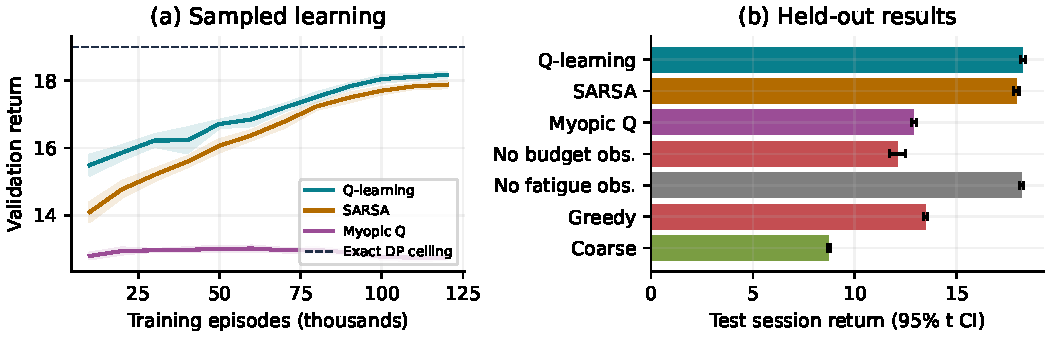
\includegraphics[width=.99\textwidth]{figures/main_results.pdf}
\captionof{figure}{Learning from sampled transitions and held-out comparisons. Shading/error bars are 95\% Student-$t$ intervals across eight seed means. The dashed line is the exact expected-return ceiling; validation and test tapes are separate.}
\label{fig:results}
\vspace{7pt}
\centering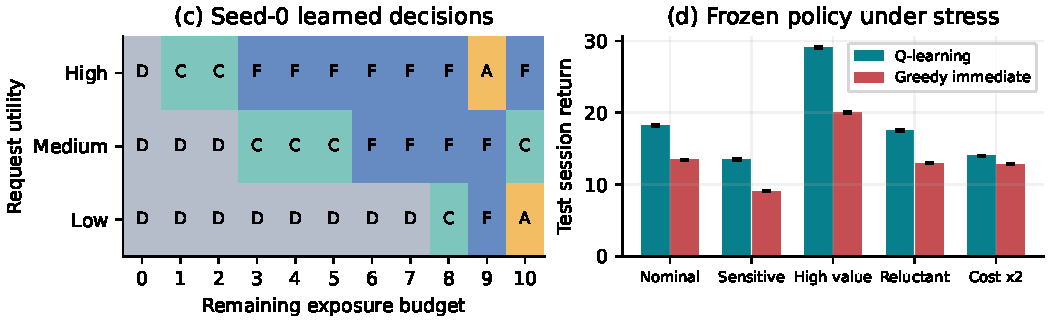
\includegraphics[width=.99\textwidth]{figures/policy_stress.pdf}
\captionof{figure}{Seed-0 decision slice and frozen-policy stress tests. D/C/A/F denote deny/coarse/ask/full. The slice fixes six requests remaining, medium sensitivity, zero fatigue, and full permission; local boundaries can be noisy. Stress bars show 95\% intervals over eight independent seed means.}
\label{fig:stress}
\vspace{9pt}
}]

\section{Results, audit, and limitations}
\begin{center}
\setlength{\tabcolsep}{3pt}\footnotesize
\begin{tabular}{@{}lrrr@{}}
\toprule
Policy & Return $\pm$95\% CI & Utility & Exposure\\
\midrule
\ResultsRows
\bottomrule
\end{tabular}
\end{center}
Q-learning achieves $\QReturn\pm\QCI$ versus greedy's $\GreedyReturn$ (paired gain $\PairedGain\pm\PairedCI$). It reaches \OptPercent\% of the exact expected optimum $\OptValue$ (estimated gap $\GapValue$). Higher utility with lower exposure than greedy supports better allocation. The sampled DP row differs slightly from its exact expectation due to test noise.

Myopic and budget-blind losses support future planning and budget observation. The fatigue-observation gain is only $\FatigueGain\pm\FatigueCI$; its interval includes zero, so these runs do \emph{not} establish a reliable marginal fatigue benefit under nominal parameters. SARSA is competitive with a lower measured mean. These results do not establish universal algorithm superiority.

\textbf{Stress and audit.} Frozen Q policies are tested separately on sensitive-heavy and high-value requests, more reluctant consent, and doubled exposure weight. Greedy knows the shifted immediate model (Figure~\ref{fig:stress}). Tests exhaustively verify feasible simulator transitions, budget/permission invariants, reward semantics, deterministic reproduction, and an independent small-MDP Monte Carlo check of exact values. The offline demo uses the saved Q table, displays visit counts, and audits a seeded session. No personal dataset is used.

\textbf{Validity limits.} Exposure units, utility trade-offs, independent requests, and consent probabilities are interpretable assumptions, not user-calibrated measurements. Coarse sharing is abstract; the budget is not differential privacy or a harm probability. Permission is observed. Disclosure composition, adversaries, real data transforms, and long-term user preferences are outside scope. Stress results apply to this synthetic family, not real users. Sparse contexts may have uncertain Q estimates. The small nominal fatigue effect is a useful negative result.

\textbf{Deliverables.} Runnable original code, environment setup, all 40 checkpoints, raw seed metrics, paired intervals, figures, hashes, tests, saved-agent demo, and editable LaTeX/PDF are included. Assistance is documented in the repository provenance note. The supplied GitHub account is labelled at the top; the actual project repository URL must replace it after publication.

\vspace{-3pt}
\begin{thebibliography}{3}\setlength{\itemsep}{-1pt}\footnotesize
\bibitem{watkins} C.~J.~C.~H. Watkins and P. Dayan. Q-learning. \emph{Machine Learning}, 8:279--292, 1992. \href{https://www.gatsby.ucl.ac.uk/~dayan/papers/cjch.pdf}{Author-hosted paper}.
\bibitem{sutton} R.~S. Sutton and A.~G. Barto. \emph{Reinforcement Learning: An Introduction}, 2nd ed. MIT Press, 2018.
\bibitem{nissenbaum} H. Nissenbaum. Privacy as contextual integrity. \emph{Washington Law Review}, 79:119, 2004. \href{https://digitalcommons.law.uw.edu/wlr/vol79/iss1/10/}{Publisher record}.
\end{thebibliography}
\end{document}
